\large\textbf{Encoder} \\[0.2em]
 Trong bài toán này, chúng ta sẽ sử dụng \textbf{Encoder} bao gồm nhiều lớp Gated Recurrent Unit, được phát minh Cho et
al. vào năm 2014. Chúng ta sẽ sử dụng GRU hai chiều, nghĩa là sẽ có 2 mạng RNN độc lập: một mạng thì đưa dữ liệu theo
chiều thuận, mạng còn lại đua theo chiều người lại. Đầu ra của mỗi mạng sẽ được cộng lại ở mỗi bước thời gian. Sử
dụng GRU hai chiều giúp mã hóa được ngữ cãnh trong tương lai và quá khứ
\begin{figure}[!htb]
    \center{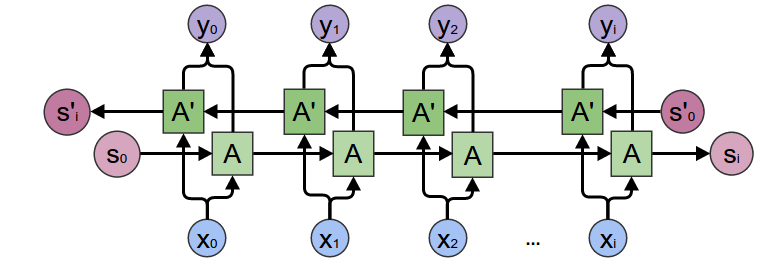
\includegraphics[width=\figureBigSize]
    {figure/model/RNN-bidirectional.png}}
    \caption{\label{fig:rnn-rolled} Recurrent Neural Network 2 chiều.}
\end{figure}

\large\textbf{Encoder} \\[0.2em]
Một vấn đề phổ biến với \textbf{Decoder} seq2seq thuần túy là chỉ dựa vào trên vectoc bối cảnh để mã hóa
toàn bộ chuỗi đầu vào có nghĩa là, có khả năng sẽ bị mất thông tin. Điều này đặc biệt xảy ra khi xử lý các chuỗi đầu
vào dài, hạn chế rất nhiều khả năng của \textbf{Decoder} .

Để chống lại điều này, Bahdanau et al. đã tạo ra một cơ chế \textbf{Attention}, cho phép bộ giải mã chú ý đến một số
phần nhất định của câu đầu vào, thay vì sử dụng toàn bộ bối cảnh cố định ở mỗi bước.

Ở mức cao, sự chú ý được tính bằng cách sử dụng trạng thái ẩn hiện tại của \textbf{Decoder} và các đầu ra của
\textbf{Encoder}. Các trọng số \textbf{Attention} đầu ra có hình dạng giống như câu đầu vào, cho phép nhân
chúng với các đầu ra của \textbf{Encoder}, cho chúng ta một tổng trọng số cho biết các phần của đầu ra
\textbf{Encoder} cần chú ý.
\begin{figure}[!htb]
    \center{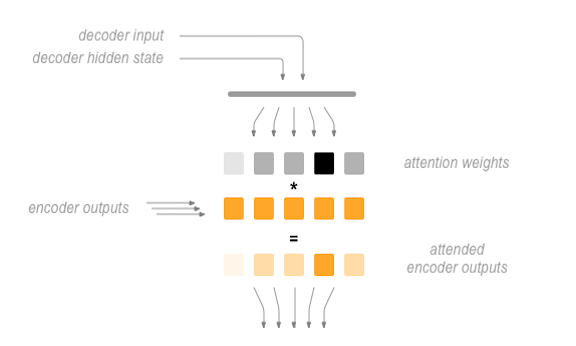
\includegraphics[width=\figureBigSize]
    {figure/model/attn2.png}}
\end{figure}

Lương Minh Thắng và cộng sự. được cải thiện dựa trên nền tảng của Bahdanau và cộng sự bằng cách tạo ra \textbf{Global
attention}. Sự khác biệt chính là với \textbf{Global attention}, xem xét tất cả các trạng thái ẩn của
\textbf{Encoder}, trái ngược với \textbf{Local attention} của Bahdanau và cộng sự. Một điểm khác biệt nữa là với
\textbf{Global attention} là tính toán trọng số chú ý hoặc năng lượng, chỉ sử dụng trạng thái ẩn của
\textbf{Encoder} từ bước thời gian hiện tại. \textbf{Local attention} của Bahdanau và cộng sự, đòi hỏi phải có thông
tin về trạng thái \textbf{Decoder} từ bước trước. Ngoài ra, Thắng còn cung cấp các phương pháp khác nhau để tính
toán năng lượng chú ý giữa đầu ra \textbf{Encoder} và đầu ra \textbf{Decoder}  được gọi là các hàm điểm số của điểm số:
\begin{figure}[!htb]
    \center{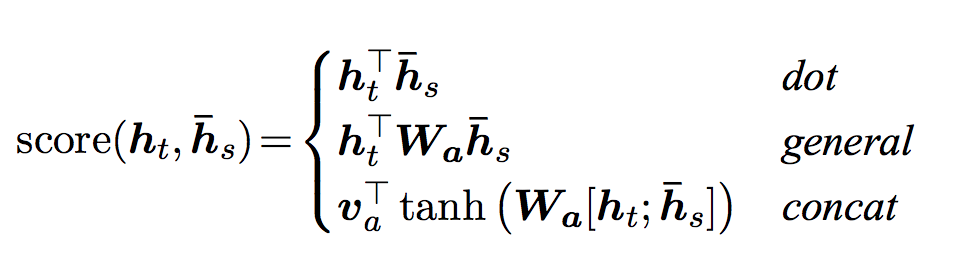
\includegraphics[width=\figureBigSize]
    {figure/model/scores.png}}
\end{figure}
\textit{Trong đó h_t là trạng thái của h_t hiện tại, \bar(h_s) là trạng thái của encoder}

Tóm lại cơ chế \textbf{Global attention} có thể biểu diễn bằng hình sau
\begin{figure}[!htb]
    \center{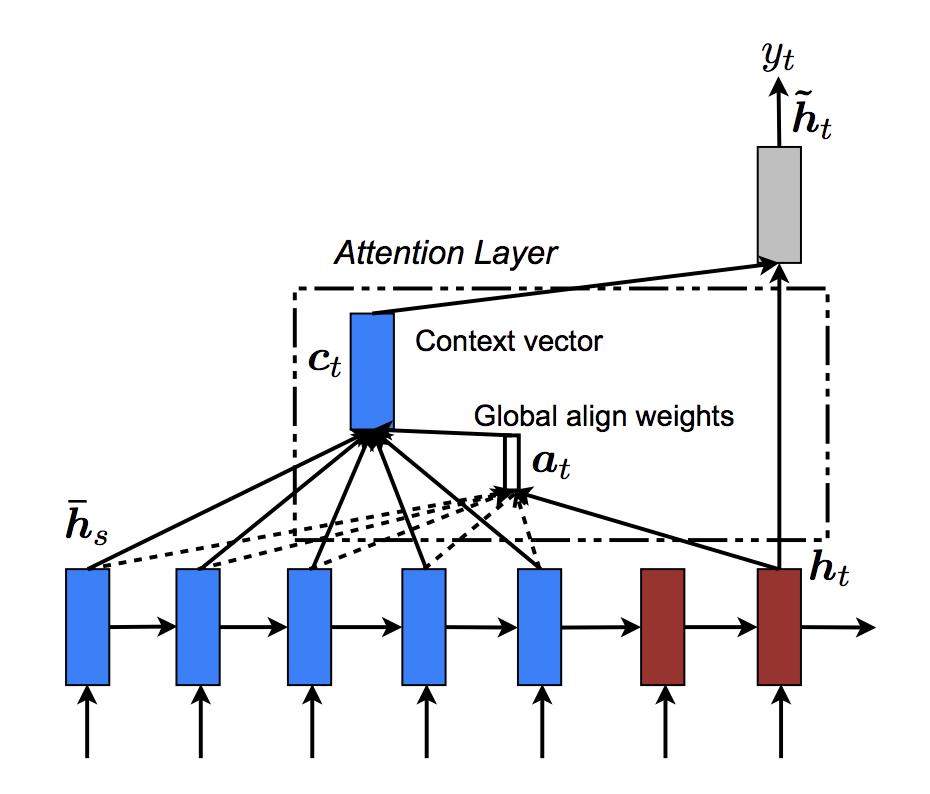
\includegraphics[width=\figureBigSize]
    {figure/model/global_attn.png}}
\end{figure}